\documentclass[a4paper,12pt]{article}
\usepackage{graphicx, xcolor}
\usepackage{geometry}
\usepackage{eso-pic}
\usepackage{cancel}
\usepackage{amsmath}
\usepackage[spanish]{babel} 
\geometry{left=2.5cm,top=3cm,bottom=3cm,right=2.5cm}

\begin{document}

\begin{titlepage}
    \newgeometry{left=2.5cm,top=1cm,bottom=2.5cm,right=2.5cm}
    \AddToShipoutPicture*{\put(0,0){\includegraphics[scale=1]{figuras/background}}} % Image background
    \noindent
    \begin{figure}
        \centering
        
\includegraphics[width=0.4\linewidth]{Logo UNC.png}
    \end{figure}
    \begin{center}
        {\scshape\Large\textbf{UNIVERSIDAD NACIONAL DE C\'ORDOBA} \par}
        \vspace{0.5cm}
        {\large{FACULTAD DE CIENCIAS EXACTAS, F\'ISICAS Y NATURALES} \par}
        \vspace{0.5cm}
        {\large{C\'ATEDRA DE S\'INTESIS DE REDES ACTIVAS} \par}
        \vspace{2cm}
        {\scshape\Huge \textbf{TRABAJO PR\'ACTICO N\textsuperscript{o} 3} \par}
        \vspace{2cm}
        {\itshape\Large "DISE\~NO DE AMPLIFICADORES" \par}
        \vspace{3cm}
        \vfill
        \begin{minipage}[t]{8cm}
            {\Large \textbf{Autores:} \par}
            {\Large Beierbach, Alejo \par}
            {\Large Ramirez, Valentin José \par}
            {\Large Lopez, Franco \par}
            {\Large Lopez Sivilat, José Ignacio \par}
        \end{minipage}\hfill\begin{minipage}[t]{8cm}
            \begin{flushright}
                {\Large \textbf{Profesores:} \par}
                {\Large Ing. Ferreyra, Pablo\par}
                {\Large Ing. Reale, Cesar\par}
            \end{flushright}
        \end{minipage}
        \vspace{1cm}
    \end{center}
\end{titlepage}

\thispagestyle{empty}
\vspace{0,2cm}
\tableofcontents

\newpage
    \vspace{3cm}
    \section{Introducción}
    \vspace{0,2cm}
\hspace{1mm}En este trabajo de laboratorio, se analizarán tres circuitos: 
\begin{enumerate}
	\item Amplificador VFA - VFA.
	\item Amplificador VFA - CFA.
	\item Amplificador VFA - CFA con red de compensación.
\end{enumerate}
\vspace{0,2cm}
\hspace{1mm}Para cada circuito, se realizará un análisis teórico, simulaciones y se compararan los resultados obtenidos.

\section{Objetivos}
\vspace{0,2cm}
\begin{itemize}
	\item Diseñar amplificadores utilizando tecnologías VFA (Amplificador Realimentado por Tensión) y CFA (Amplificador Realimentado por Corriente) aplicando conceptos de compensación.
	\item Fortalecer el uso del simulador LTspice.
	\item Comparar los errores relativos que existen entre el modelo teórico calculado y las simulaciones.
	
\end{itemize}
\section{Desarrollo}
\vspace{0,2cm}
\hspace{1mm}La figura 1 muestran un amplificador compuesto que deberá ser diseñado para obtener una
ganancia global Avf = 20dB, compensándolo para obtener una máxima planicidad de módulo
($M\varphi =65^\circ$ o Qp = 0, 707).
\begin{figure}[h] 
    \centering
    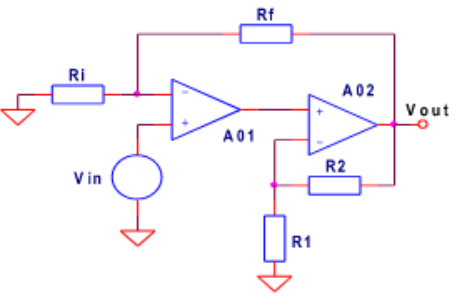
\includegraphics[width=0.5\linewidth]{Circuito1.png}
    \caption{Esquema del amplificador compuesto}
    \label{fig:enter-label}
\end{figure}
\newpage
\subsection{Amplificador VFA - VFA:}
\vspace{0,2cm}
\hspace{1mm}Las especificaciones del VFA LM324 se detallan a continuaci\'on.

\begin{itemize}
    \item $A_{d0}=100~dB$
    \item $f_T=1~MHz$
    \item $f_1=10~Hz$
    \item $f_2=5.06~MHz$
\end{itemize}
\vspace{0,2cm}
\hspace{1mm}Considerando AO2 como ideal, se calcularan las ganancias de lazo abierto $Ad(s)$, ganancia de lazo $T(s)$ y ganancia de lazo cerrado $Avf(s)$.\\
\vspace{0.2cm}
\hspace{1mm}A continuacion en la Figura 2 se muestra donde se corta el lazo.
\begin{figure}[h]
    \centering
    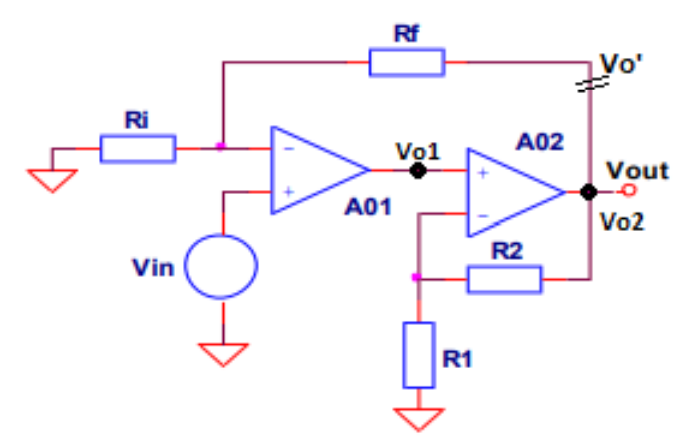
\includegraphics[width=0.5\linewidth]{CircuitoLazoAbierto.png}
    \caption{Esquema del amplificador compuesto lazo abierto}
    \label{fig:enter-label}
\end{figure}
\subsubsection{Ganancia de Lazo Abierto}
\vspace{0,2cm}
\hspace{1mm}Es la relación entre la tensión de salida y la tensión de entrada.

\begin{equation}
    Av(s) = \frac{V_{out}}{V_{in}}|_{V_{o'}=0}  
\end{equation}
\vspace{0,2cm}
\hspace{1mm}Por un lado, se tiene

\begin{equation}
    V_{o1} = Ad(s)\cdot V_{in} 
\end{equation}
\vspace{0,2cm}
\hspace{1mm}Además

\begin{equation}
    V_{o} = \left(1+\frac{R_2}{R_1}\right) \cdot V_{o1} 
    \end{equation}
\begin{equation}    
    V_{o} = \left(1+\frac{R_2}{R_1}\right) \cdot Ad(s) \cdot V_{in}
\end{equation}

\vspace{0,2cm}
\hspace{1mm}Por lo tanto

\begin{equation}
\boxed{Av(s) = \left(1+\frac{R_2}{R_1}\right) \cdot Ad(s)}
\end{equation}
\subsubsection {Ganancia de Lazo T}
\vspace{0,2cm}

\begin{equation}
    T(s) = \frac{V_{out}}{V_{o'}}|_{V_{in}=0}
    \end{equation}
    
\begin{equation}
    T(s) = \left(1+\frac{R_2}{R_1}\right) \cdot (-Ad(s)) \cdot \left(\frac{R_i}{R_i+R_f}\right)
\end{equation}
\vspace{0,2cm}
\hspace{1mm}Entonces,
\begin{equation}
 \boxed{T(s) = -Ad(s) \cdot \left(1+\frac{R_2}{R_1}\right) \cdot \left(\frac{R_i}{R_i+R_f}\right)}
\end{equation}

\subsubsection {Ganancia de Lazo Cerrado}
\vspace{0,2cm}
\begin{equation}
    Avf(s) = \frac{Av(s)}{1-T}
\end{equation}
\vspace{0,2cm}
\hspace{1mm}Reemplazando se llega a
\begin{equation}
     Avf(s) = \frac{\left(1+\frac{R_2}{R_1}\right) \cdot Ad(s)}{1+Ad(s) \cdot \left(1+\frac{R_2}{R_1}\right) \cdot \left(\frac{R_i}{R_i+R_f}\right)} \label{eq:primera} \\
   \nonumber
     = \frac{\left(1+\frac{R_2}{R_1}\right)}{\frac{1}{Ad(s)} + \left(1+\frac{R_2}{R_1}\right) \cdot \left(\frac{R_i}{R_i+R_f}\right)} 
\end{equation}
\vspace{0,2cm}
\hspace{1mm}Considerando la ganancia $Ad(s)$ que tiende a ser muy grande o infinita, se simplifican los cálculos

\begin{equation}
    Avf(s) = \frac{\cancel{\left(1+\frac{R_2}{R_1}\right)}}{\cancel{\left(1+\frac{R_2}{R_1}\right)} \cdot \left(\frac{R_i}{R_i+R_f}\right)} 
\end{equation}
\vspace{0,2cm}
\hspace{1mm}Por lo tanto

\begin{equation}
    \boxed{Avf(s)=\frac{R_i+R_f}{R_i}}
\end{equation}

\vspace{0,2cm} 
\hspace{1mm}La consigna define que la ganancia de lazo cerrado debe ser $Avf(s)=20~dB$. Con dicho dato, es posible obtener la relación entre las resistencias $R_i$ y $R_f$.

\begin{equation}
    Avf(s)=20~dB \hspace{5mm}\hspace{5mm} \frac{R_i+R_f}{R_i}=20~dB = 10~veces
\end{equation}

\vspace{0,2cm}
\hspace{1mm}Despejando la relación de resistencias,

 
\begin{equation}
    \frac{R_f}{R_i} = 9
\end{equation}

\vspace{0,2cm}
\hspace{1mm}Colocando valores arbitrarios de resistencias para cumplir con la relaci\'on, se llega a:

\begin{align}
    R_i &= 10~\text{k}\Omega \\ 
    R_f &= 90~\text{k}\Omega
\end{align}
\vspace{0,2cm}
\hspace{1mm}Considerando el producto ancho de banda-frecuencia constante, obtenemos:

\begin{equation}
   f_g*10=100000*10Hz
\end{equation}
\begin{equation}
   f_g=100KHz
\end{equation}

\vspace{0,2cm}
\hspace{1mm}Con este valor calculado, se determin\'o la ganancia a lazo cerrado del amplificador AO2 ideal. Recordando que la consigna especificaba que $Avfi=20~dB$ y que $Ad_o=100~dB$:

\begin{align}
    Avf_{2i}&=\frac{Avfi \cdot \omega_{gi}}{Ad_0 \cdot \omega_1} =\frac{10~veces \cdot 2\pi\cdot 100 ~KHz}{100~Kveces\cdot 2\pi\cdot10~Hz} \label{eq:primera} \\
   \nonumber
   \\
    Avf_{2i}&=1~veces =0~dB
\end{align}

\vspace{0,2cm}
\hspace{1mm}Siendo $ \omega _1 $ la frecuencia del primer polo, especificada en frecuencia angular. Finalmente, la ganancia del amplificador compuesto resulta

\begin{equation}
    Av_{comp}=Ad0\cdot Avf_{2i}=100~dB \cdot 0~dB
\end{equation}

\begin{equation}
    \boxed{
    Av_{comp} = 100~dB
    }
\end{equation}
\vspace{0,2cm}
\hspace{1mm}En este punto, es posible obtener el valor de las resistencias $R_1$ y $R_2$

\begin{equation}
    Avf_{2i}=0~dB \hspace{5mm}\hspace{5mm} \frac{R_1+R_2}{R_1}=0~dB = 1~veces
\end{equation}
\vspace{0,2cm}
\hspace{1mm}Entonces

\begin{equation}
    R_1>>R_2
\end{equation}
\vspace{0,2cm}
\hspace{1mm}Colocando valores arbitrarios de resistencias para cumplir con la relación, se llega a:

\begin{equation}
    \boxed{
    \begin{aligned}
        &R_1=100~K\Omega \\
        &R_2=1~K\Omega
    \end{aligned}
    }
\end{equation}

\subsubsection{Simulaciónes}
\vspace{0,2cm}
\hspace{1mm}Digrama de bode realizado con Phyton en Figura 3:
\begin{figure}
    \centering
    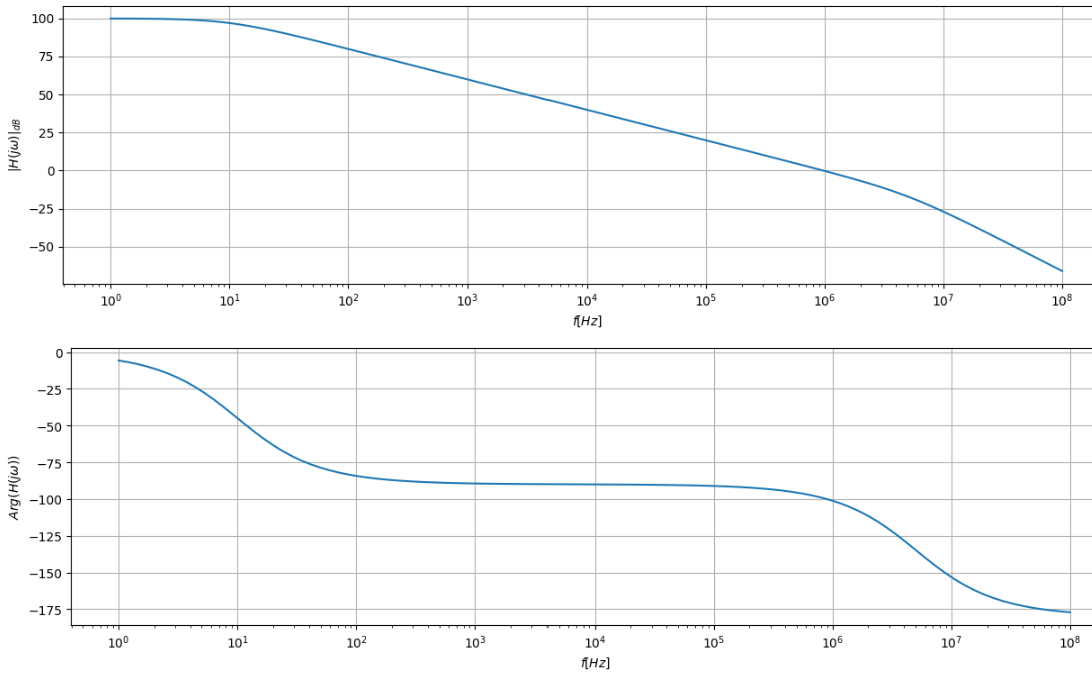
\includegraphics[width=0.9\linewidth]{BodeVFA-VFA.png}
    \caption{Diagrama de bode}
    \label{fig:enter-label}
\end{figure}
\newpage
\hspace{1mm}Circuito simulado con LTspice:
\begin{figure}[h]
    \centering
    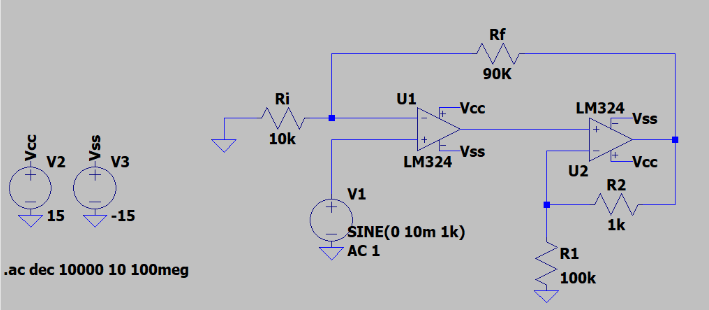
\includegraphics[width=0.9\linewidth]{CircuitoVFA_VFA-LTspice.png}
    \caption{Circuito en LTspice}
    \label{fig:enter-label}
\end{figure}

\hspace{1mm} Ganancia del amplificador compuesto y respuesta en frecuencia:
\begin{figure}
    \centering
    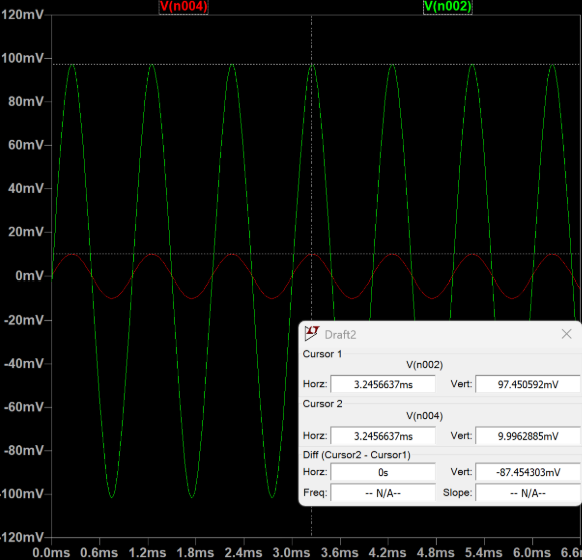
\includegraphics[width=0.7\linewidth]{Vin-Vout_VFA-VFA.png}
    \caption{Ganancia}
    \label{fig:enter-label}
\end{figure}
\begin{figure}
    \centering
    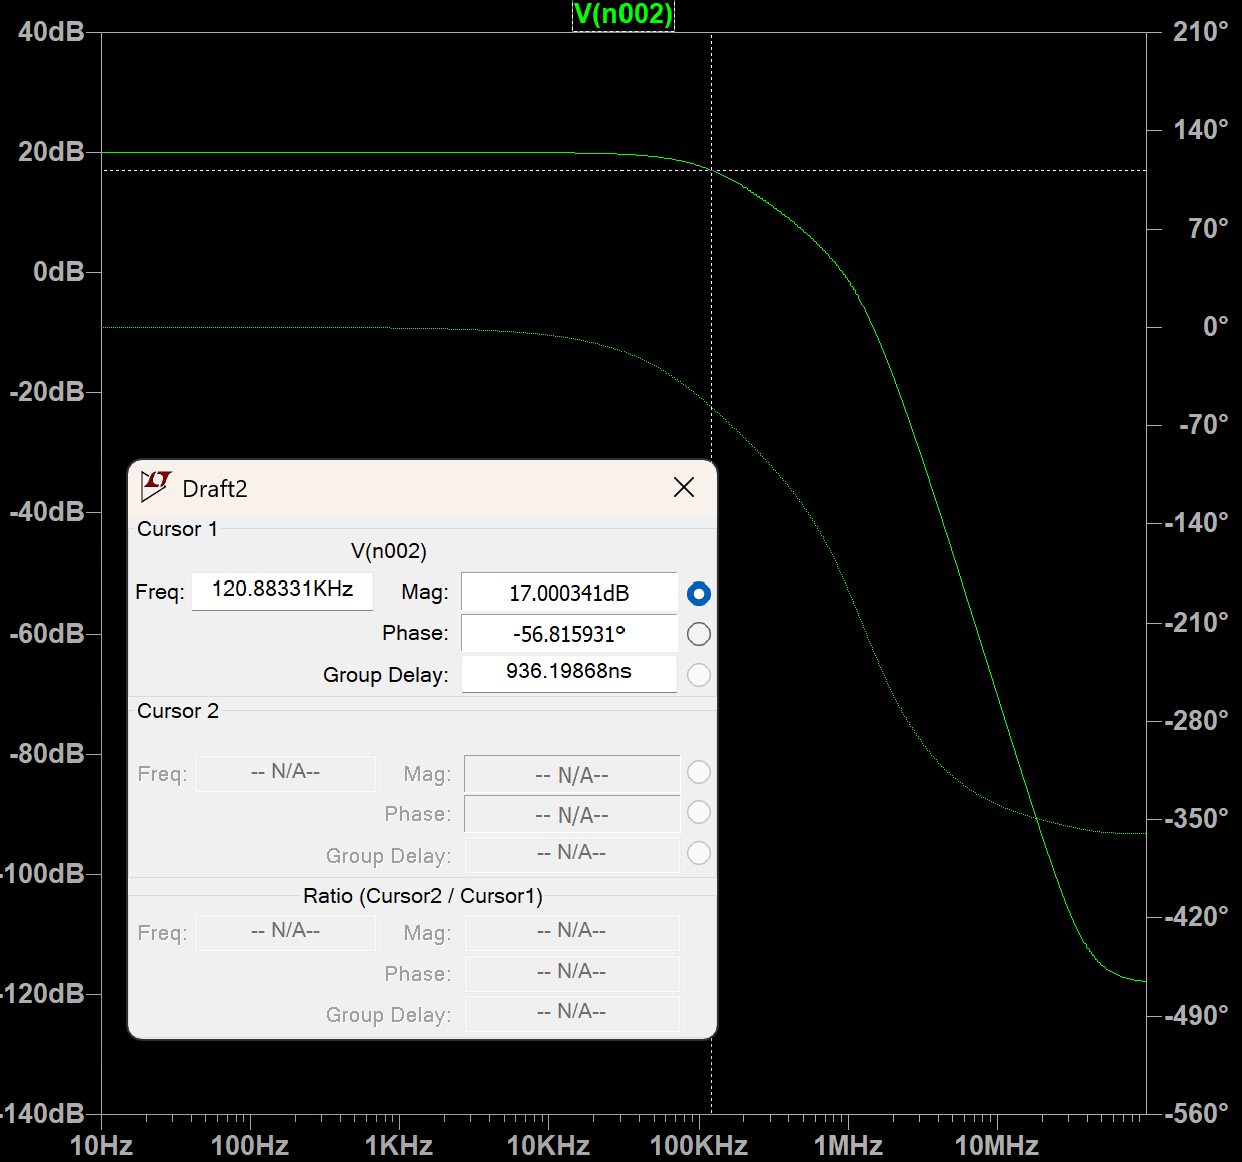
\includegraphics[width=0.7\linewidth]{RTAenF_VFA-VFA.png}
    \caption{Respuesta en frecuencia}
    \label{fig:enter-label}
\end{figure}
\newpage
\subsubsection{Conclusiones}
\vspace{0.2cm}
\hspace{1mm}De las simulaciones obtenemos que los valores de ganancia del circuito y la frecuencia de corte son los siguientes:
\begin{equation}
    {Avf(s)=\frac{97.45~mV}{10~mV}}=9,745~veces
\end{equation}
\begin{equation}
f_g=120~KHz
\end{equation}
\vspace{0,2cm}
\hspace{1mm}Por lo que el error porcentual en la ganancia a lazo cerrado es de:
\begin{equation}
    E_\%=\frac{|10-9.745|}{9.745}*100=2.62\%
\end{equation}
\hspace{1mm}El error porcentual de la frecuencia de corte es de:
\begin{equation}
    E_\%=\frac{|100~KHz-120KHz|}{120~KHz}*100=16,67\%
\end{equation}
\vspace{0,2cm}
\hspace{1mm}En conclusion los errores obtenidos son aseptables y se permite validar el diseño del circuito VFA-VFA
\newpage
\subsection{Amplificador VFA - CFA:}
\vspace{0,2cm}
\hspace{1mm}Para el desarrollo de este caso, se utilizar\'a el mismo circuito propuesto en el apartado anterior, pero se reemplazar\'a el A02 por un CFA. Se decidi\'o actualizar el amplificador operacional CFA propuesto en la consigna, reemplazando el LM6181 por el AD8011 de ANALOG DEVICE debido a su obsolescencia.\\\\
\hspace{1mm}Las especificaciones del VFA LM324 se detallan a continuaci\'on.

\begin{itemize}
    \item $A_{d0}=100~dB$
    \item $f_T=1~MHz$
    \item $f_1=10~Hz$
    \item $f_2=5,06~MHz$
\end{itemize}
\vspace{0,2cm}
\hspace{1mm}Las especificaciones del CFA AD8011 se detallan a continuaci\'on.
\begin{itemize}
    \item $R_T=450~K\Omega$
    \item $C_T=2,3~pF$
\end{itemize}

\subsubsection{Análisis teórico}
\vspace{0,2cm}
\hspace{1mm}Para el desarrollo de este caso, se considerará que el VFA presenta el mismo comportamiento que el caso anterior. Además, el polo de mayor frecuencia del CFA cuenta con un efecto despreciable sobre la respuesta del amplificador a lazo cerrado.
Con ello, la ecuación del margen de fase para máxima planicidad resulta:

\begin{equation}
    M \varphi = 180^o - arctg \left(\frac{f_g}{f_{1VFA}}\right) - arctg \left(\frac{f_g}{f_{2VFA}}\right) - arctg \left(\frac{f_g}{f_{CFA}}\right) = 65,5^o
\end{equation}
\vspace{0.2cm}
\hspace{1mm}Reemplazando por los valores que son dato.

\begin{equation}
    65,5^o = 180^o - arctg \left(\frac{2~MHz}{10~Hz}\right) - arctg \left(\frac{2~MHz}{5,06~MHz}\right) - arctg \left(\frac{2~MHz}{f_{CFA}}\right)
\end{equation}
\vspace{0.2cm}
\hspace{1mm}Dado que el polo $ f_{1VFA} $ se encuentra lo suficientemente alejado como para no influir sobre la respuesta del amplificador
\begin{equation}
    \Longrightarrow arctg \left(\frac{2~MHz}{10~Hz}\right) = 90^o
\end{equation}
\vspace{0.2cm}
\hspace{1mm}Entonces

\begin{equation}
    65,5^o = 180^o - 90^o - 21,57^o - arctg \left(\frac{2~MHz}{f_{CFA}}\right)
\end{equation}
\vspace{0,2cm}
\hspace{1mm}Resolviendo y despejando se obtiene.

\begin{equation}
    tg (2,93^o) = \frac{2~MHz}{f_{CFA}}
\end{equation}
\vspace{0,2cm}
\hspace{1mm}Entonces, para obtener una máxima planicidad, la frecuencia del polo de lazo cerrado del CFA debe ser

\begin{equation}
    f_{CFA} = \frac{2~MHz}{tg (2,93^o)}
\end{equation}
\begin{equation}
     \boxed{
        f_{CFA} = 39~MHz
    }
\end{equation}
\vspace{0,2cm}
\hspace{1mm}Contando con dicha frecuencia, se procede a calcular la resistencia $ R_2 $ partiendo de la siguiente ecuación:

\begin{equation}
    \omega _{CFA} = \frac{1}{C_T \cdot R_2}
\end{equation}


\begin{align}
   \Longrightarrow R_2 &= \frac{1}{C_T \cdot 2\pi f_{CFA}}
    \\
    R_2 &= \frac{1}{2,3~pF \cdot 2\pi \cdot 39~MHz}
\end{align}

\begin{equation}
    \boxed{
        R_2 = 1774~\Omega=> 1800~\Omega
    }
\end{equation}
\vspace{0,2cm}
\hspace{1mm}Para calcular la resistencia $ R_1 $ se parte del producto ganancia por ancho de banda.
\begin{equation}
    Avf \cdot f_g = Ado \cdot f_1 \cdot Avf_2
\end{equation}
\vspace{0.2cm}
\hspace{1mm}donde $ Avf_2 $ es la ganancia ideal de lazo cerrado del CFA. Despejando la fórmula anterior

\begin{align}
   \Longrightarrow Avf_2 &= \frac{Avf \cdot f_g}{Ado \cdot f_1} \label{eq:primera} \\
   \nonumber
   \\
         &= \frac{10 \cdot 2~MHz}{100000 \cdot 10~Hz}
\end{align}

\begin{equation}
    \boxed{
    Avf_2 = 20
    }
\end{equation}

\vspace{0,2cm}
\hspace{1mm}Recordando que 

\begin{equation}
    Avf_2 = 1 + \frac{R_2}{R_1} = 20
\end{equation}

\vspace{0,2cm}
\hspace{1mm} Se despeja $ R_1 $ de la ecuación anterior

\begin{align}
   \Longrightarrow R_1 &= \frac{R_2}{Avf_2 - 1} \label{eq:primera} \\
   \nonumber
   \\ 
                       &= \frac{1800~\Omega}{20 - 1}
\end{align}

\begin{equation}
    \boxed{
    R_1 = 94,74~\Omega=>100~\Omega
    }
\end{equation}

\bigskip
\subsubsection{Simulaciones}
\vspace{0,2cm}
\hspace{1mm}Nuevamente en este apartado, se simuló el circuito final para evaluar los cálculos obtenidos con anterioridad. El circuito utilizado fue el siguiente:
\begin{figure}[h]
    \centering
    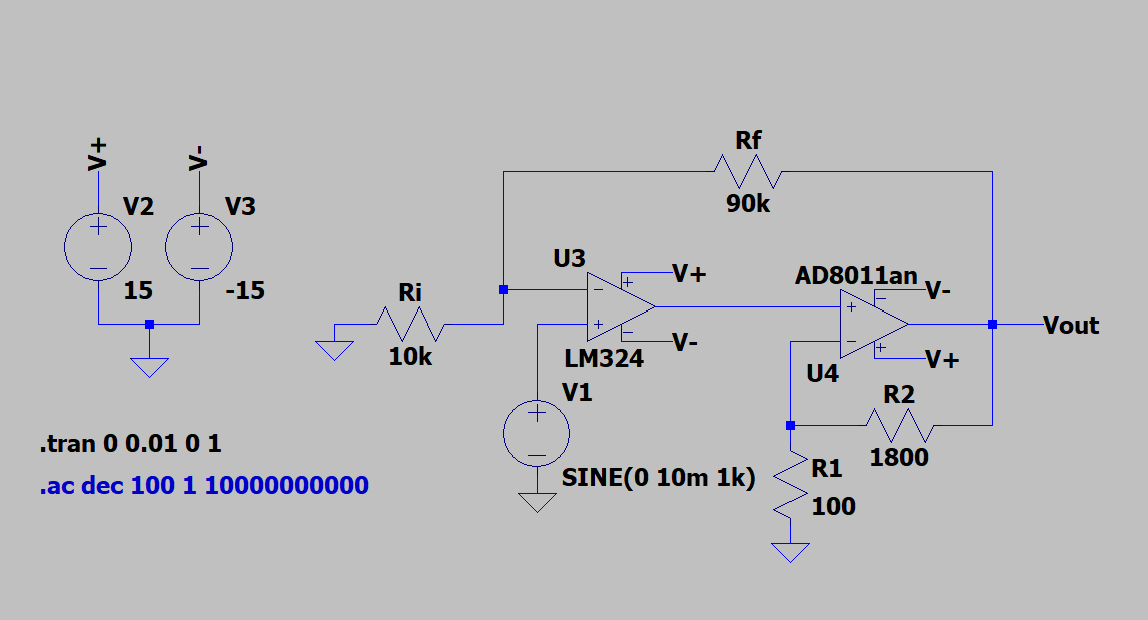
\includegraphics[width=1\linewidth]{CircuitoVFA_CFA_I.png}
    \caption{Circuito VFA-CFA en LTspice}
    \label{fig:enter-label}
\end{figure}
\\
\hspace{1mm}Ganancia del amplificador compuesto y respuesta en frecuencia:
\begin{figure}
    \centering
    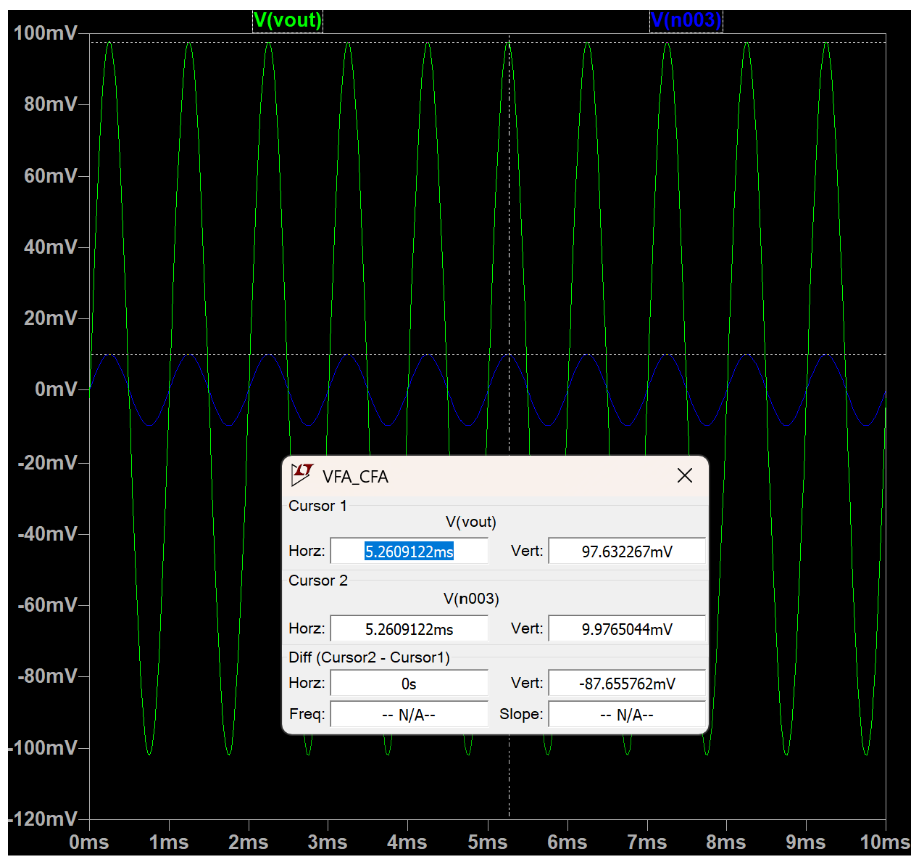
\includegraphics[width=0.7\linewidth]{Ganancia_circuito2.png}
    \caption{Ganancia del circuito VFA-CFA}
    \label{fig:enter-label}
\end{figure}
\begin{figure}
    \centering
    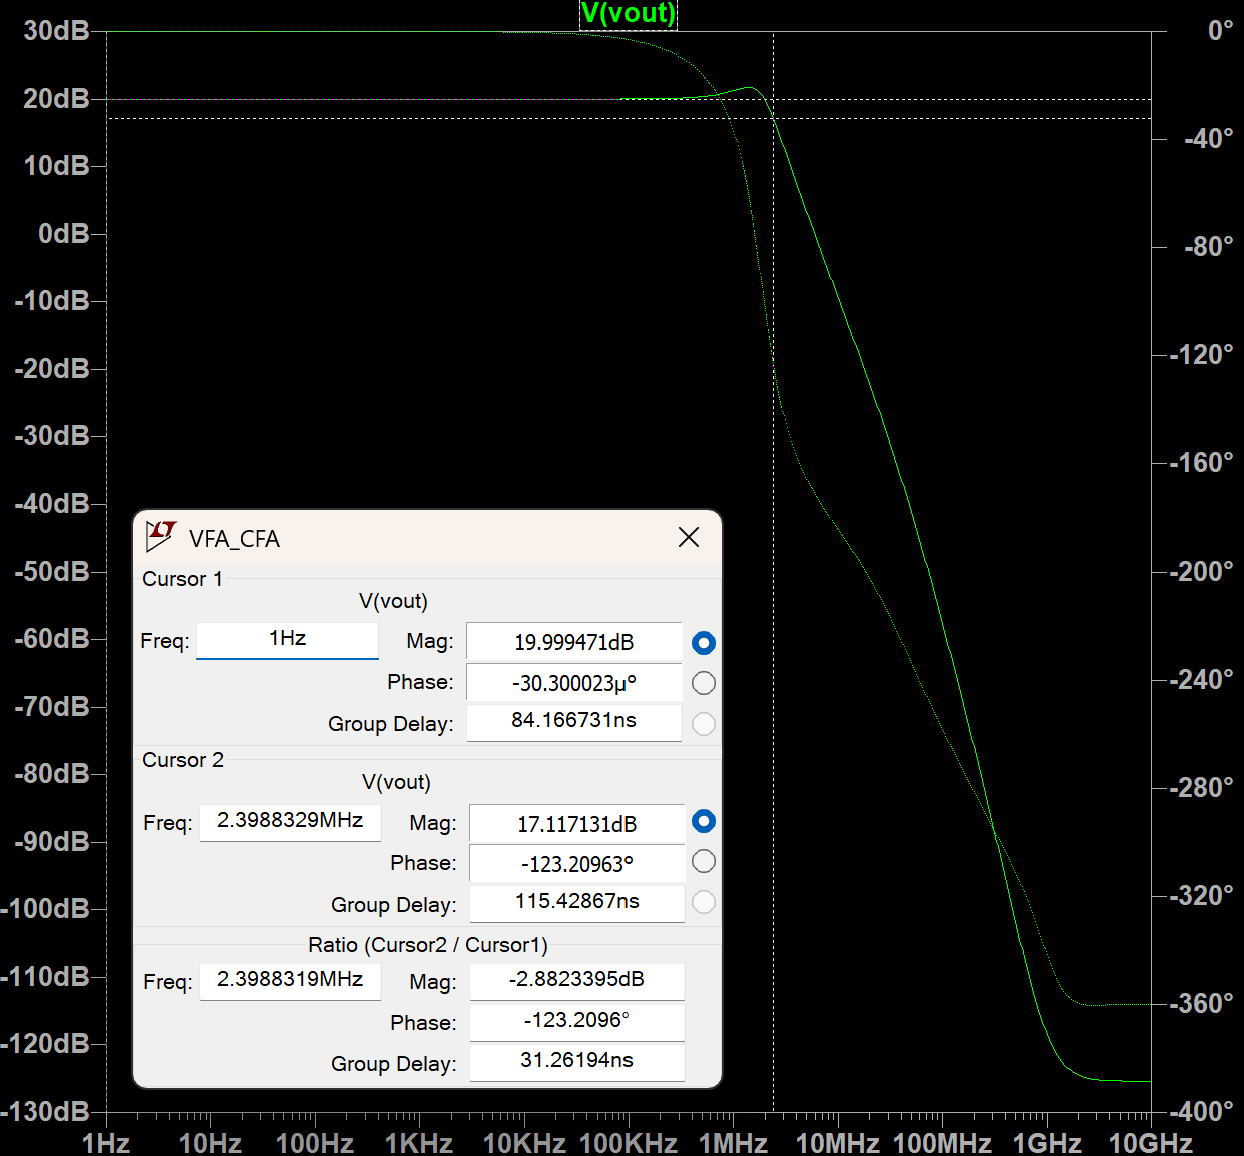
\includegraphics[width=0.7\linewidth]{RTA_VFA-CFA-I.png}
    \caption{Respuesta en frecuencia del circuito VFA-CFA}
    \label{fig:enter-label}
\end{figure}
\newpage
\subsubsection{Conclusión}
\vspace{0,2cm}
\hspace{1mm}De las simulaciones obtenemos que los valores de ganancia del circuito y la frecuencia de corte son los siguientes:
\begin{equation}
    {Avf(s)=\frac{97.63~mV}{10~mV}}=9,76~veces
\end{equation}
\begin{equation}
f_g=2,4~MHz
\end{equation}
\vspace{0.2cm}
\hspace{1mm}Por lo que el error porcentual en la ganancia a lazo cerrado es de:
\begin{equation}
    E_\%=\frac{|10-9.76|}{9.76}*100=2.46\%
\end{equation}
\vspace{0,2cm}
\hspace{1mm}El error porcentual de la frecuencia de corte es de:
\begin{equation}
    E_\%=\frac{|2~MHz-2,4~MHz|}{2,4~KHz}*100=8,33\%
\end{equation}
\hspace{1mm}En conclusion los errores obtenidos son aseptables y se permite validar el diseño del circuito VFA-CFA\\
\newpage
\subsection{Amplificador VFA - CFA II:}
\vspace{0.5cm}
\hspace{1mm}En este apartado se procede a anadir una red de compensaci\'on cero-polo a la configuraci\'on anterior, con
el prop´osito espec\'ifico de cancelar el polo ubicado en 5,06 MHz del amplificador VFA.
\begin{figure}[h]
    \centering
    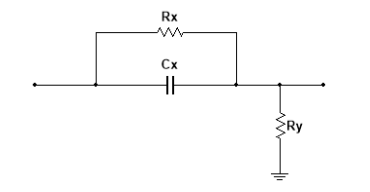
\includegraphics[width=0.5\linewidth]{Red_Compensacion.png}
    \caption{Red de compensaci\'on RC cero-polo}
    \label{fig:enter-label}
\end{figure}
\vspace{0.5cm}
\subsubsection{Análisis teórico}
\vspace{0.2cm}
\hspace{1mm}La red de compensaci\'on cuenta con la siguiente función transferencia 

\begin{equation}
    A_c(s) = \frac{R_y}{R_x + R_y} \cdot \frac{1 + sC_x R_x}{1 + sC_x (R_x // R_y)}
\end{equation}
\vspace{0.2cm}
\hspace{1mm}Donde se definen las siguientes notaciones:

\begin{itemize}
    \item $k_{comp}=\frac{R_y}{R_x + R_y}$
    \item $ \omega_{pcomp} =  \frac{1 }{1 + sC_x (R_x // R_y)}$
    \item $\omega_{zcomp} = \frac{1 }{ C_xR_x}$
\end{itemize}
\vspace{0.2cm}
\hspace{1mm}Dado que el cero del compensador debe cancelar el polo producido por $f_2$, se tendr\'a

\begin{equation}
    \Longrightarrow \omega_{zcomp} = \omega_2 = 2\pi \cdot 5.06~Mrps
\end{equation}
\vspace{0.2cm}
\hspace{1mm}Como se solicit\'o en la consigna, el polo de compensación se ubicar\'a una octava por encima de este cero, resultando entonces:

\begin{equation}
    \omega _{pcomp} = 2\cdot\omega _{zcomp} = 2\pi \cdot 10.12~Mrps 
\end{equation}
\vspace{0.2cm}
\hspace{1mm}Con estos valores deducidos, es posible calcular la ganancia del compensador

\begin{equation}
    k_{comp} = \frac{\omega_{zcomp}}{\omega _{pcomp}} = \frac{2\pi \cdot 5.06~Mrps}{2\pi \cdot 10.12~Mrps}
\end{equation}

\begin{equation}
    \boxed{
    k_{comp} = 0.5
    }
\end{equation}
\vspace{0.2cm}
\hspace{1mm}Recordando que

\begin{equation}
    k_{comp} = \frac{R_y}{R_x + R_y}  \Longrightarrow  ~ \frac{R_y}{R_x + R_y} = 0.5
\end{equation}
\vspace{0.2cm}
\hspace{1mm}Despejando para obtener la relación entre las resistencias
\begin{align}
    \frac{R_y}{R_x + R_y} &= \frac{1}{2}        \\
                     2R_y &= R_x + R_y           \\
                        2 &= \frac{R_x}{R_y} + 1
\end{align}

\begin{equation}
    \boxed{
    1 = \frac{R_x}{R_y}
    }
\end{equation}
\vspace{0.2cm}
\hspace{1mm}Considerando valores normales 

\begin{equation}
    \boxed{
    R_x = R_y = 1~k\Omega
    }
\end{equation}
\vspace{0.2cm}
\hspace{1mm}Obtenido el valor de las resistencias, es posible calcular el valor del capacitor $C_x$, despejando de la ecuación del cero 

\begin{equation}
    \begin{aligned}
              \omega_{zcomp} &= \frac{1}{C_x R_x}                     \\
        \Longrightarrow C_x &= \frac{1}{\omega_{zcomp} \cdot {R_x}}  \\
                        C_x &= \frac{1}{2\pi \cdot 5.06~Mrps \cdot 1~k\Omega}
    \end{aligned}
\end{equation}

\begin{equation}
    \boxed{
    C_x = 31~pF
    }
\end{equation}
\vspace{0.2cm}
\hspace{1mm}Al agregar el compensador, se obtiene la siguiente función de transferencia del lazo de realimentación:

\begin{equation}
    \begin{aligned}
        T(s) &= -A_d(s) \cdot A_c(s) \cdot A_{vf2} (s)\\
             &= - \frac{k\cdot A_d(0)}{\left(1+\frac{s}{\omega_1}\right)\left(1+\frac{s}{\omega_2}\right)} \cdot k_{comp} \frac{\left(1 + \frac{s}{\omega_{zcomp}}\right)}{\left(1+\frac{s}{\omega_{pcomp}}\right)} \cdot A_{vf2}(s)
    \end{aligned}
\end{equation}

\vspace{0.2cm}
\hspace{1mm} donde:
\begin{itemize}
    \item $k:$ realimentación del VFA.
    \item $A_d(0):$ ganancia del VFA.
    \item $A_{vf2}:$ función de transferencia del CFA.
    \item $ \omega_1 , \omega_2 :$ los polos del VFA.
\end{itemize}
\vspace{0.2cm}
\hspace{1mm}Se observa que el valor de $k_{comp}$ induce una atenuación en la función de transferencia, y por ende, en la ganancia. Por ello, es necesario ajustar la ganancia a lazo cerrado del CFA, teniendo en cuenta que $ k_{comp} = 0.5 $:

\begin{equation}
    A_{vf2 comp} (s) = 2\cdot A_{vf2}(s)
\end{equation}
\vspace{0.2cm}
\hspace{1mm}Esta relaci\'on garantiza que la atenuaci\'on provocada por $k_{comp}$ se compense adecuadamente en la ganancia a lazo cerrado del Compensador de Fase Avanzada (CFA), asegurando así un rendimiento equilibrado del sistema. Recordando que $A_{vf2}$ es:

\begin{equation}
    A_{vf2} = 1 + \frac{R_2}{R_1}
\end{equation}
\vspace{0.2cm}
\hspace{1mm}Reemplazando se obtiene.

\begin{equation}
    \begin{aligned}
        A_{vf2 comp} (s) &= 2 \left( 1 + \frac{R_2}{R_1} \right)\\
             &= 2 \cdot 20
    \end{aligned}
\end{equation}

\begin{equation}
    \boxed{
    A_{vf2 comp} (s) = 40
    }
\end{equation}
\vspace{0.2cm}
\hspace{1mm}Dado que el polo del CFA permanece invariable con respecto al caso anterior, el valor de $R_2$ continúa siendo 

\begin{equation}
    \boxed{
    R_2 = 1800~\Omega
    }
\end{equation}
\vspace{0.2cm}
\hspace{1mm}Por su parte, $R_1$ se obtiene de:

\begin{equation}
    \begin{aligned}
        \frac{R_2}{R_1} &= 40 - 1 \\
    \Longrightarrow R_1 &= \frac{1800~\Omega}{39}
    \end{aligned}
\end{equation}

\begin{equation}
    \boxed{
    R_1 = 46,15~\Omega=>47~\Omega
    }
\end{equation}
\bigskip
\subsubsection{Simulaciones}
\hspace{0,2cm}
\hspace{1mm}Nuevamente en este apartado, se simul\'o el circuito final para evaluar los cálculos obtenidos con anterioridad. El circuito utilizado fue el siguiente:
\begin{figure}
    \centering
    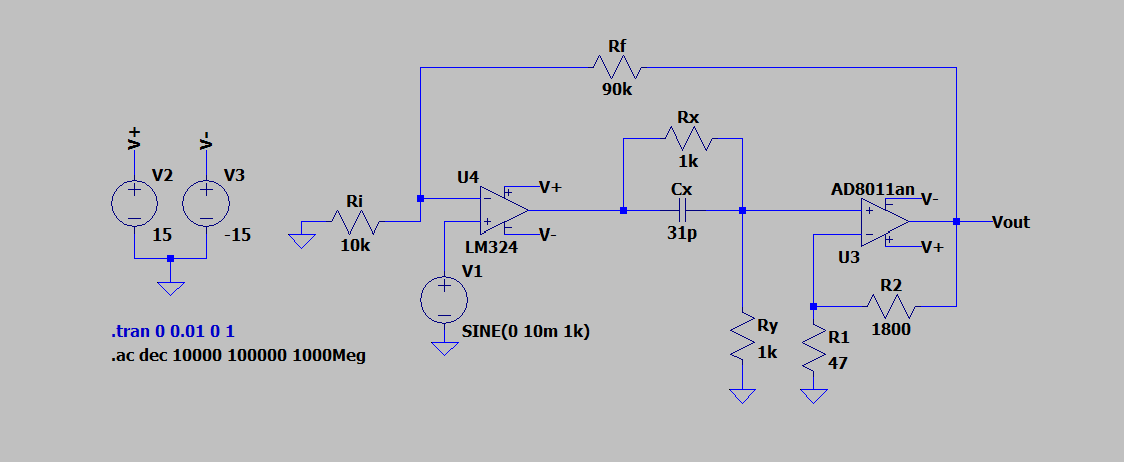
\includegraphics[width=1\linewidth]{Circuito_VFA-CFA-II.png}
    \caption{Circuito VFA-CFA compensado en LTspice}
    \label{fig:enter-label}
\end{figure}
\hspace{1mm}Ganancia del amplificador compuesto y respuesta en frecuencia:
\begin{figure}
    \centering
    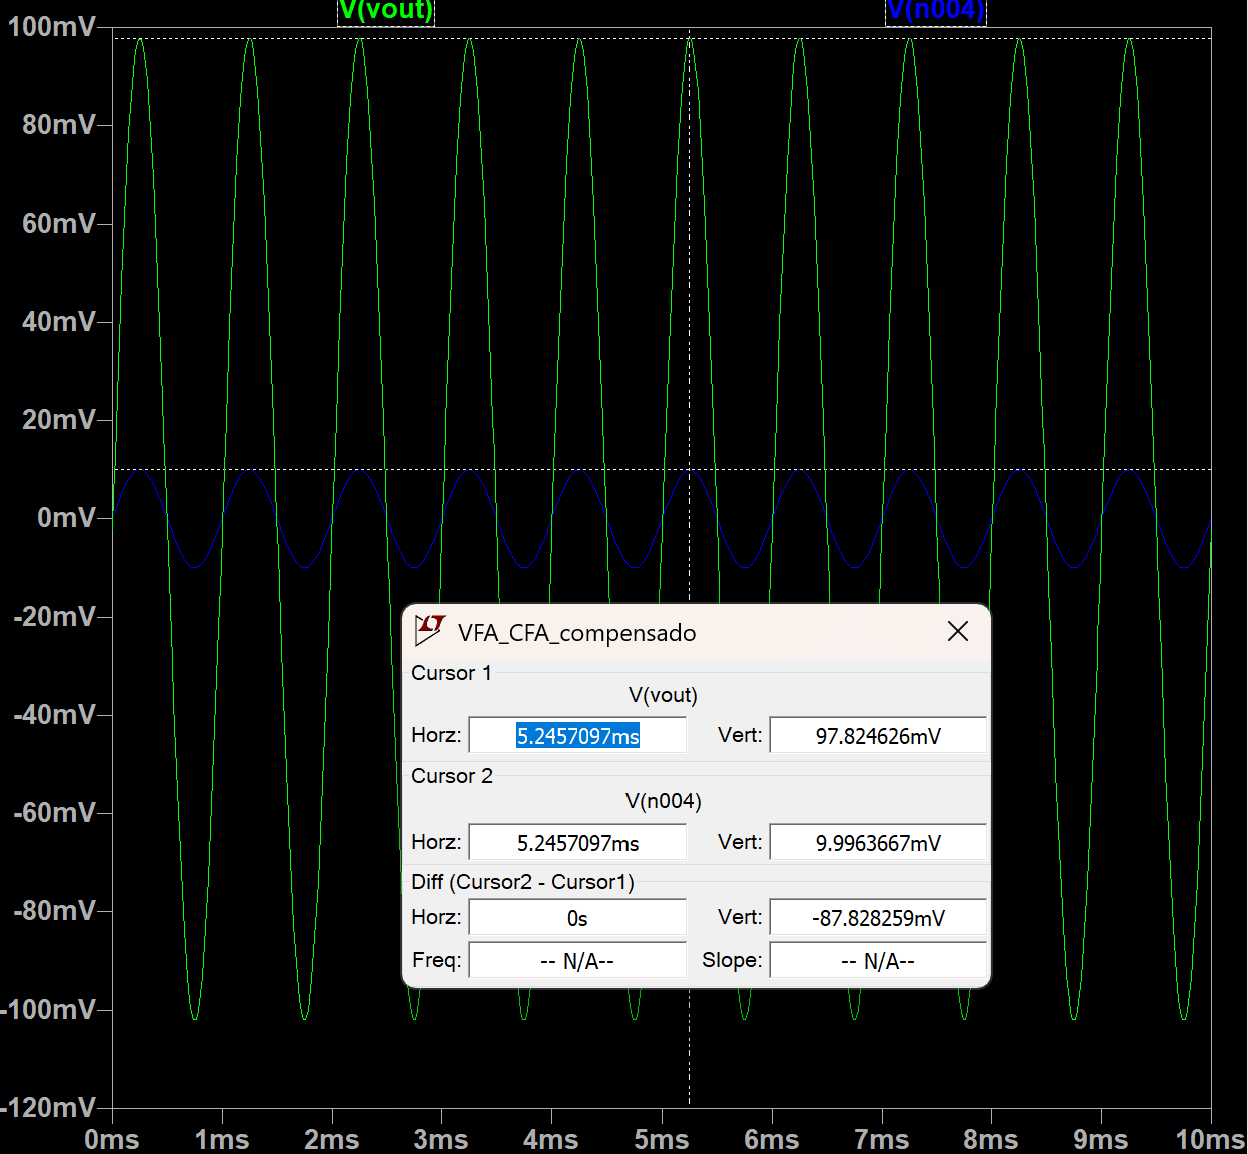
\includegraphics[width=0.7\linewidth]{Ganancia_VFA-CFA-II.png}
    \caption{Ganancia del circuito VFA-CFA compensado}
    \label{fig:enter-label}
\end{figure}

\begin{figure}
    \centering
    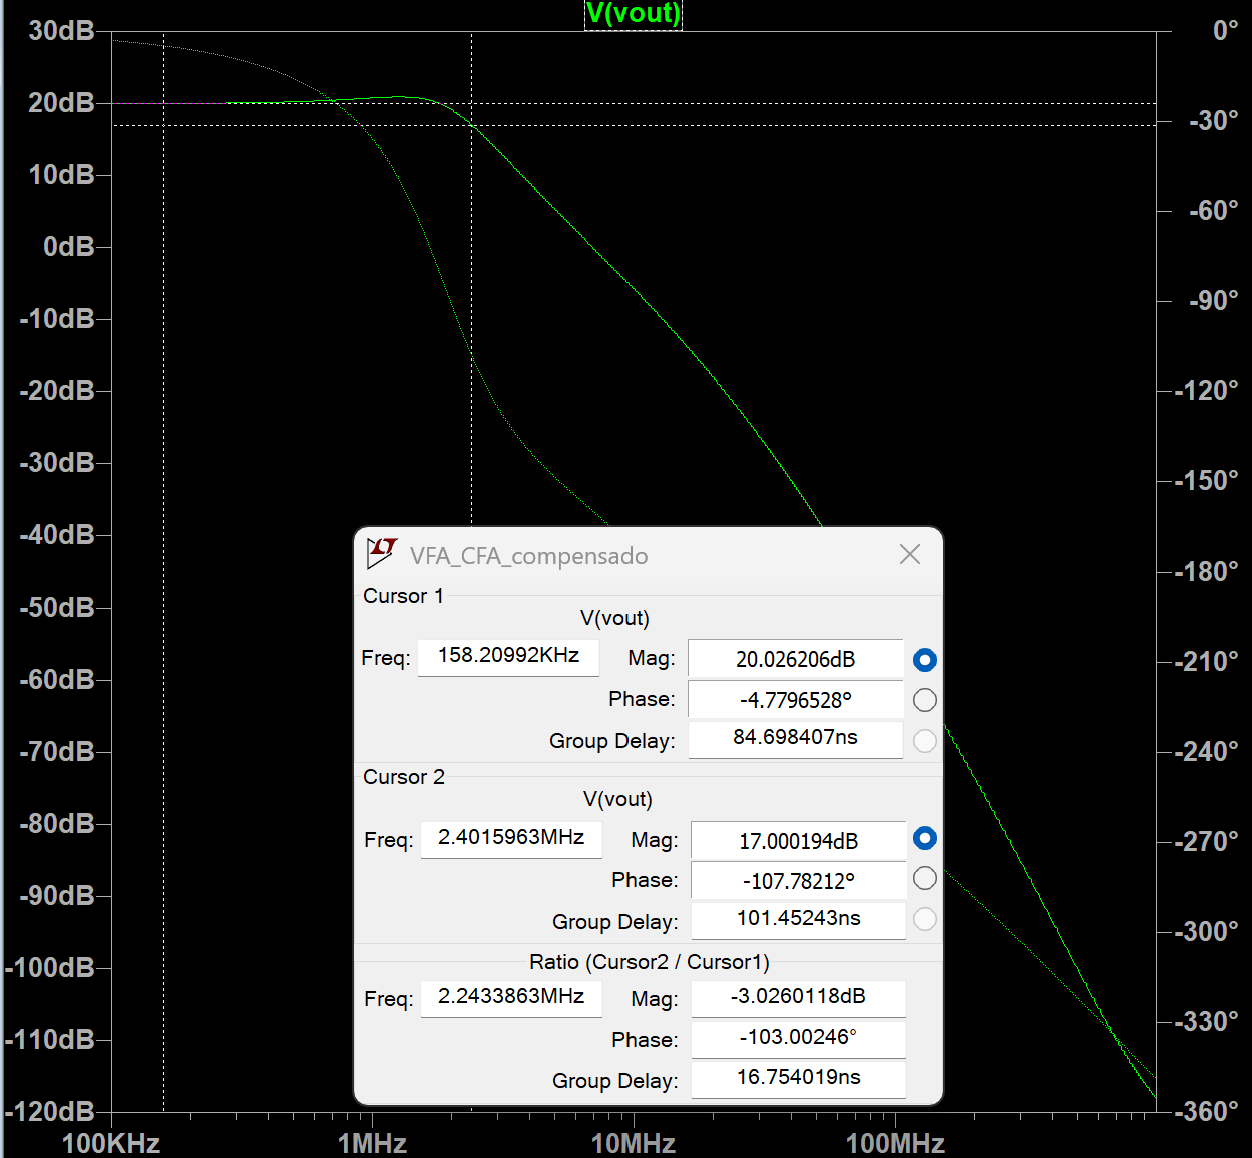
\includegraphics[width=0.7\linewidth]{RTA_VFA-CFA-II.png}
    \caption{Respuesta en frecuencia del circuito VFA-CFA compensado}
    \label{fig:enter-label}
\end{figure}
\newpage
\subsubsection{Conclusiones}
\vspace{0.2cm}
\hspace{1mm}De las simulaciones obtenemos que los valores de ganancia del circuito y la frecuencia de corte son los siguientes:
\begin{equation}
    {Avf(s)=\frac{97.82~mV}{10~mV}}=9,8~veces
\end{equation}
\begin{equation}
f_g=2,4~MHz
\end{equation}
\vspace{0,2cm}
\hspace{1mm}Por lo que el error porcentual en la ganancia a lazo cerrado es de:
\begin{equation}
    E_\%=\frac{|10-9.8|}{9.8}*100=2\%
\end{equation}
\hspace{1mm}El error porcentual de la frecuencia de corte es de:
\begin{equation}
    E_\%=\frac{|2~MHz-2,4~MHz|}{2,4~KHz}*100=8,33\%
\end{equation}
\hspace{1mm}En conclusion los errores obtenidos son aseptables y se permite validar el diseño del circuito VFA-CFA compensado. Además este circuito dismuniye el pico de ganancia en la frecuencia de corte y disminuye el error en la ganancia total.\\

\end{document}
